\section{Evaluation}
\label{sec:eval}

This section evaluates the performance gains and preparation costs of local optimizations implemented with \kinsns. We measure execution time with computational microbenchmarks, examine throughput in complete applications, and compare local optimization with whole-program native compilation. We address four questions:

\begin{itemize}
\item \textbf{RQ1:} How much do local optimizations reduce eBPF program execution time?
\item \textbf{RQ2:} How much do these optimizations improve application throughput?
\item \textbf{RQ3:} What additional costs do program rewriting and first loading introduce?
\item \textbf{RQ4:} How do local optimization and whole-program native compilation compare for applications?
\end{itemize}

\noindent\textbf{Experimental setup.}
We run x86-64 experiments on EC2 c7i.large instances with Intel Xeon Platinum 8488C processors. The ARM64 experiments use c7g.large instances with AWS Graviton3 processors. Both instance types provide two vCPUs and run our research kernel based on Linux 7.0.0-rc2. Within each architecture, all program configurations use the same kernel and module builds. The microbenchmarks use the programs, inputs, and platforms from \S\ref{sec:characterization}. Application workloads are described in their respective subsections.

\subsection{Microbenchmark Performance}
\label{subsec:micro_benchmark}

We use the 27 computational microbenchmarks from \S\ref{sec:characterization} to distinguish the performance gains from recompilation and from rewriting computations as \kinsns. The eBPF JIT baseline directly loads bytecode generated by Clang 18.1.3 at \texttt{-O2}. \tool recompiles the same bytecode in user space and uses the pattern recognizer to introduce \kinsns. We also run \tool without \kinsn rewriting, disabling the rules that introduce these instructions. Both \tool configurations use the same modified LLVM 23 compiler, with O3 IR optimization and \texttt{Aggressive} backend code generation.

All three paths execute programs through the kernel's \texttt{BPF\_PROG\_TEST\_RUN} interface. We use 12 independent instances per architecture, interleave measurements of the three paths within each instance, and collect ten readings per program and path after warmup. We compare mean execution time per invocation, excluding rewriting and loading.

\begin{figure*}[t]
\centering
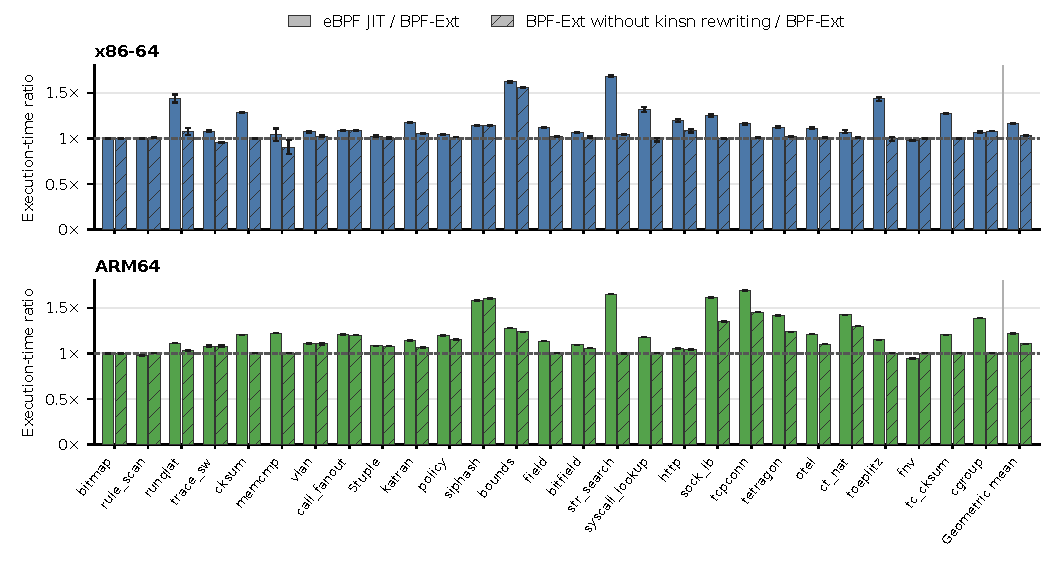
\includegraphics[width=\textwidth]{figures/sec-6-micro-performance.pdf}
\caption{Execution-time ratios for the microbenchmarks in Table~\ref{tab:microbenchmarks}. Ratios are the reference configuration's mean execution time divided by that of \tool{}. Values above 1 indicate faster execution with \tool{}. Disabling \kinsn rewriting preserves the LLVM configuration. Geometric mean summarizes the 27 ratios. Error bars show 95\% confidence intervals from paired resampling of independent instances.}
\Description{Two panels show execution-time ratios for x86-64 and ARM64 across 27 benchmarks and their geometric means. Solid bars compare eBPF JIT with BPF-Ext. Hatched bars compare BPF-Ext without kinsn rewriting with BPF-Ext. The dashed horizontal line marks equal execution time.}
\label{fig:eval-kinsn-micro}
\end{figure*}

Rewriting computations as \kinsns improves performance beyond recompilation alone. Figure~\ref{fig:eval-kinsn-micro} reports both comparisons. Relative to the eBPF JIT, \tool achieves geometric-mean speedups of 1.17$\times$ on x86-64 and 1.22$\times$ on ARM64. Relative to \tool without \kinsn rewriting, the speedups are 1.04$\times$ and 1.11$\times$, respectively. The full pipeline's gains therefore include both recompilation and \kinsn rewriting. Across the same 27 programs, the geometric mean of native code size falls by 15.1\% and 12.9\% relative to the eBPF JIT.

The benefit of \kinsn rewriting varies across programs. For example, the x86-64 string-search benchmark, \texttt{str\_search}, achieves a 1.68$\times$ speedup over the eBPF JIT but only 1.05$\times$ over \tool without \kinsn rewriting. Most of its overall gain is already present in the common compilation pipeline. ARM64 SipHash instead gains mainly from \kinsn rewriting, with corresponding speedups of 1.58$\times$ and 1.60$\times$.

A rotation ablation further identifies the benefit of this optimization in ARM64 SipHash. We disable only the rotation rule, keeping the compilation pipeline and all other rules unchanged. With rotation enabled, native rotation instructions replace 116 combinations of shifts and bitwise OR, while eight memory-access extensions remain unchanged between configurations. In a separate experiment with 12 independent instances, mean execution time falls from 121.2\,ns with rotation disabled to 77.1\,ns with rotation enabled, a 1.57$\times$ speedup and a 36.4\% reduction in execution time.

\subsection{Application Performance}
\label{subsec:corpus_application}

\begin{table*}[t]
\centering
\small
\caption{Applied optimizations in each \tool application configuration. The last column lists categories of \kinsns actually generated, using the names in Section~\ref{subsec:operations}.}
\label{tab:eval-application-configurations}
\setlength{\tabcolsep}{5pt}
\renewcommand{\arraystretch}{1.08}
\begin{tabular*}{\textwidth}{@{\extracolsep{\fill}}ll>{\raggedright\arraybackslash}p{0.48\textwidth}@{}}
\toprule
\textbf{Application} & \textbf{Configuration} & \textbf{Applied optimizations} \\
\midrule
Cilium & All optimizations & Address calculation, conditional select,\newline bulk memory access, prefetch \\
 & Without bulk memory access & Address calculation, conditional select, prefetch \\
\addlinespace
Katran & Register optimizations & Rotation, bit extraction \\
 & Register and memory optimizations & Rotation, bit extraction, big-endian load,\newline bulk memory access, prefetch \\
\bottomrule
\end{tabular*}
\end{table*}

\begin{table*}[t]
\centering
\small
\caption{Application throughput in millions of packets accepted by the sending interfaces per second (Mpps). Relative rates divide each configuration's mean by the application's eBPF JIT mean. Brackets give 95\% confidence intervals.}
\label{tab:eval-application-throughput}
\setlength{\tabcolsep}{5pt}
\renewcommand{\arraystretch}{1.08}
\begin{tabular*}{\textwidth}{@{\extracolsep{\fill}}llrc@{}}
\toprule
\textbf{Application} & \textbf{Configuration} & \textbf{Mean (Mpps)} & \textbf{Relative rate [95\% CI]} \\
\midrule
Cilium & eBPF JIT & 0.575 & 1.000 \\
 & All optimizations & 0.557 & 0.970 [0.871, 1.093] \\
 & Without bulk memory access & 0.575 & 1.000 [0.932, 1.075] \\
\addlinespace
Katran & eBPF JIT & 1.722 & 1.000 \\
 & Register optimizations & 1.710 & 0.993 [0.988, 0.998] \\
 & Register and memory optimizations & 1.721 & 0.999 [0.993, 1.005] \\
\bottomrule
\end{tabular*}
\end{table*}

\begin{table*}[t]
\centering
\small
\caption{Katran CPU costs from independent sampling. Entries give the median across three instances, with the minimum and maximum in parentheses. Estimated CPU time is divided by the increase in the virtual-IP packet counter over the same sending window. Application + callees includes kernel functions attributed to Katran through its call stacks.}
\label{tab:eval-katran-profile}
\setlength{\tabcolsep}{3pt}
\renewcommand{\arraystretch}{1.08}
\begin{tabular*}{\textwidth}{@{\extracolsep{\fill}}lcc@{}}
\toprule
\textbf{Configuration} & \textbf{Application code (ns/packet)} & \textbf{Application + callees (ns/packet)} \\
\midrule
eBPF JIT & 116.3 (114.8--118.3) & 260.4 (259.8--265.4) \\
Register optimizations & 121.5 (119.9--126.6) & 261.0 (260.6--268.5) \\
Register and memory optimizations & 121.3 (110.8--123.2) & 260.6 (259.3--269.9) \\
\bottomrule
\end{tabular*}
\end{table*}


We test whether these local optimizations improve packet-processing throughput in complete applications. Cilium~\cite{cilium} exercises a network datapath with multiple eBPF programs and tail calls, while Katran~\cite{katran} exercises XDP load balancing. Cilium uses version 1.20.0-dev on x86-64, with bidirectional IPv4 UDP traffic between two endpoints. Katran runs on ARM64, forwarding traffic from one UDP virtual IP address to one backend. Both workloads use 64-byte packets generated by two pktgen threads, each configured with 65,535 flows.

For each application, we compare the eBPF JIT with two \tool configurations. Cilium enables either all seven optimization categories in \S\ref{subsec:operations}, or the same set without bulk memory access and its associated recognition rules. Katran enables three register optimizations: rotation, conditional select, and bit extraction. A second configuration adds three memory optimizations: big-endian load, bulk memory access, and prefetch. Table~\ref{tab:eval-application-configurations} lists the categories of \kinsns actually generated under these configurations. Katran's two configurations rewrite 21 and 68 sites, respectively.

We measure application throughput after the service and datapath are ready, using 12 independent instances per configuration. Each Cilium instance warms up for 180 seconds before three 180-second measurement windows, with the Cilium agent paused during measurement. Katran uses a 30-second warmup followed by three 30-second windows. The main measurements disable BPF runtime statistics and CPU sampling. Throughput is the sum of the rates of packets accepted by the transmitting interface, as reported by the two pktgen threads. We average the three windows within each instance, then aggregate the 12 instance experiments. We compute 95\% confidence intervals for throughput ratios by jointly resampling 12 experiment batches, each containing a separate instance for every configuration.

Table~\ref{tab:eval-application-throughput} reports throughput relative to the eBPF JIT. For Cilium, enabling all optimizations yields 0.970 times the throughput obtained without bulk memory access (95\% confidence interval: [0.874, 1.083]). For Katran, adding memory optimizations to the register optimizations yields a throughput ratio of 1.006 (95\% confidence interval: [0.997, 1.015]).

To measure where CPU time is spent, we sample application code and the kernel functions it calls in separate experiments. For each Katran configuration, three fresh instances each warm up for 30 seconds before a 30-second traffic experiment with sampling. Table~\ref{tab:eval-katran-profile} reports the results. Cilium's corresponding samples appear alongside the native-compilation comparison in \S\ref{subsec:native-comparison}.

\subsection{Rewriting and First-Load Cost}
\label{subsec:preparation-cost}

\begin{table*}[t]
\centering
\small
\caption{Rewriting and first-load costs in milliseconds, using the same LLVM pipeline with and without \kinsn rewriting. Entries summarize per-program means across 27 programs. Ranges give the minimum and maximum across programs. Increments are computed per program as the cost with rewriting minus the cost without it, before summarization.}
\label{tab:eval-preparation-cost}
\setlength{\tabcolsep}{5pt}
\renewcommand{\arraystretch}{1.08}
\begin{tabular*}{\textwidth}{@{\extracolsep{\fill}}lrrrr@{}}
\toprule
 & \multicolumn{2}{c}{\textbf{x86-64}} & \multicolumn{2}{c}{\textbf{ARM64}} \\
\cmidrule(lr){2-3}\cmidrule(l){4-5}
\textbf{Measurement} & \textbf{Median} & \textbf{Range} & \textbf{Median} & \textbf{Range} \\
\midrule
Without \kinsn rewriting & 24.0 & 15.4--109.8 & 24.2 & 13.9--145.7 \\
With \kinsn rewriting & 35.6 & 24.4--138.9 & 34.2 & 23.8--155.7 \\
Per-program increment & 9.2 & 3.6--46.2 & 10.0 & 2.6--15.7 \\
\bottomrule
\end{tabular*}
\end{table*}


Local optimization adds work before program execution, so we measure the combined cost of rewriting and first loading. Using the 27 programs from \S\ref{subsec:micro_benchmark}, we compare \tool with and without \kinsn rewriting. Starting from existing bytecode, the timed stages cover userspace rewriting, reading the rewritten program, and the first object load. Object loading includes extension-target resolution and the program-loading call, which performs kernel verification and JIT compilation.

Rewriting and first loading typically take tens of milliseconds in the current implementation. Table~\ref{tab:eval-preparation-cost} summarizes the mean costs of the 27 programs. With \kinsn rewriting, the median cost is 35.6\,ms on x86-64 and 34.2\,ms on ARM64. The median per-program increase over the configuration without \kinsn rewriting is 9.2\,ms and 10.0\,ms, respectively.

The typical additional cost comes mainly from the loader's lookup of kernel implementations for \kinsns. The current loader resolves BTF information afresh on each load, taking a median of 9.1\,ms across programs on x86-64 and 9.9\,ms on ARM64. In comparison, the median increase in userspace rewriting time is 0.12\,ms and 0.14\,ms. Some x86-64 programs are recompiled after checks of rewriting conditions, adding to rewriting cost. The Katran microbenchmark's 46.2\,ms increase includes 36.6\,ms of rewriting.

Program loading is also a substantial part of preparation cost. For the string-search benchmark, which has the highest total cost, the program-loading call takes 85.8\,ms on x86-64 and 121.8\,ms on ARM64. These times include libbpf processing, kernel verification, and JIT compilation.

\subsection{Whole-Program Native Comparison}
\label{subsec:native-comparison}

\begin{table}[ht]
\centering
\small
\caption{Cilium throughput ratios, using mean rates of packets accepted by the sending interfaces. Each ratio divides whole-program native throughput by the reference throughput. Brackets give 95\% confidence intervals.}
\label{tab:eval-native-comparison}
\setlength{\tabcolsep}{3pt}
\renewcommand{\arraystretch}{1.08}
\begin{tabular}{@{}lc@{}}
\toprule
\textbf{Reference} & \textbf{Native / reference} \\
\midrule
eBPF JIT & 1.005 [0.939, 1.098] \\
All optimizations & 1.036 [0.931, 1.141] \\
Without bulk memory access & 1.005 [0.952, 1.065] \\
\bottomrule
\end{tabular}
\end{table}

\begin{table*}[t]
\centering
\small
\caption{Cilium CPU costs from independent sampling. Entries give the median across three instances, with the minimum and maximum in parentheses. Estimated CPU time is divided by packets accepted by the sending interfaces over the same sending window. Map operations include their internal callees attributed to Cilium through call stacks.}
\label{tab:eval-cilium-profile}
\setlength{\tabcolsep}{5pt}
\renewcommand{\arraystretch}{1.08}
\begin{tabular*}{\textwidth}{@{\extracolsep{\fill}}lcc@{}}
\toprule
\textbf{Configuration} & \textbf{Application code (ns/packet)} & \textbf{Map operations (ns/packet)} \\
\midrule
eBPF JIT & 208.5 (191.2--227.9) & 1,065.2 (1,027.3--2,233.9) \\
All optimizations & 198.2 (189.3--213.3) & 1,093.8 (1,050.0--1,960.8) \\
Whole-program native & 186.9 (186.1--188.6) & 1,074.6 (1,072.4--1,200.5) \\
\bottomrule
\end{tabular*}
\end{table*}


We use whole-program native compilation as a reference to compare local optimization with broader compiler optimization in an application. This experiment uses the same Cilium version and configuration as \S\ref{subsec:corpus_application}, compiles its BPF source directly to native code, and adapts the calling convention, helper calls, context access, and configuration access. Native compilation uses Clang 18.1.3 at \texttt{-O3}, targets Sapphire Rapids, and uses only general-purpose registers to meet kernel execution constraints.

This comparison trusts the entire native implementation and its integration code. The original eBPF program first passes kernel verification, after which the loader installs the native implementation before the program is attached. The verifier's acceptance of the eBPF program does not establish equivalence to its native implementation.

The native configuration uses the workload and throughput measurement procedure from \S\ref{subsec:corpus_application}, achieving a mean throughput of 0.578\,Mpps. Table~\ref{tab:eval-native-comparison} compares it directly with the eBPF JIT and both \tool configurations.

We also sample CPU time for the eBPF JIT, \tool with all seven optimization categories, and whole-program native compilation. Each configuration uses three fresh instances, with a 180-second warmup followed by one 180-second sampling window. Table~\ref{tab:eval-cilium-profile} reports the sampled costs of application code and map operations.